% Exercise — Structural Estimation with Deep Surrogates (single + joint)
% Rewritten for TFP-persistence single-parameter and joint SMM exercises.
\documentclass[10pt,aspectratio=169]{beamer}

\usepackage[utf8]{inputenc}
\usepackage[T1]{fontenc}
\usepackage{lmodern}
\usepackage{amsmath, amssymb, amsthm}
\usepackage{booktabs}
\usepackage{graphicx}
\usepackage{hyperref}
\usepackage{tikz}
\usepackage{xcolor}

\graphicspath{{fig/}}

\setbeamertemplate{footline}{
  \hfill
  \insertframenumber\,/\,\inserttotalframenumber\kern1em\vskip4pt}
\setbeamerfont{frametitle}{size=\huge}

% Color setup mirrored from preceding deck
\definecolor{uzhblue}{RGB}{0, 40, 165}
\definecolor{uzhgreylight}{RGB}{235, 235, 235}
\definecolor{darkred}{RGB}{170, 0, 0}
\definecolor{softblue}{RGB}{60, 100, 200}

\newcommand{\E}[1]{\mathbb{E}\!\left[#1\right]}
\newcommand{\emphc}[1]{\textbf{\textcolor{darkred}{#1}}}

\setbeamercolor{title}{fg=uzhblue}
\setbeamercolor{frametitle}{bg=uzhgreylight, fg=uzhblue}
\setbeamercolor{block title}{bg=uzhblue, fg=white}
\setbeamercolor{block body}{bg=uzhgreylight, fg=black}
\setbeamercolor{block title alerted}{bg=darkred, fg=white}
\setbeamercolor{block body alerted}{bg=uzhgreylight, fg=darkred}

\DeclareMathOperator*{\argmin}{arg\,min}

\title[SMM exercise -- Padova 2026]%
{Deep Learning for Solving Dynamic Models}
\subtitle{Session 7 (exercise): Surrogate-based structural estimation via SMM}
\author{Simon Scheidegger}
\institute[HEC Lausanne]{HEC, University of Lausanne}
\date{University of Padova\\September 24, 2026}

\begin{document}

% --- Title slide ---
{\setbeamercolor{background canvas}{bg=uzhgreylight}
\begin{frame}
\titlepage
\end{frame}
}

% --- Slide 2: model ---
\begin{frame}{The Model: Brock--Mirman with Stochastic TFP}
\small
Stochastic growth model:
\vspace{-4pt}
\[
\max_{\{C_t\}} \sum_{t=0}^{\infty} \beta^t \E{\ln C_t}, \qquad
K_{t+1} + C_t = Y_t + (1-\delta)K_t
\]
\vspace{-12pt}
\[
Y_t = z_t K_t^\alpha, \qquad \log z_{t+1} = \varrho\log z_t + \sigma\,\varepsilon_{t+1}, \qquad \varepsilon_{t+1}\sim\mathcal{N}(0,1).
\]

\textbf{Calibrated parameters}
\begin{center}\begin{tabular}{cccc}
\toprule
$\alpha$ & $\delta$ & $\sigma$ & $\beta$ (single-$\varrho$ exercise) \\
\midrule
$0.36$ & $0.10$ & $0.04$ & $0.96$ \\
\bottomrule
\end{tabular}\end{center}
\vspace{-0.05cm}
{\scriptsize Note: the textbook closed-form policy $s = \alpha\beta$ requires $\delta = 1$. We use $\delta = 0.10$, so no analytic policy exists and the Euler equation must be solved numerically -- the surrogate replaces this expensive inner solve.}

\textbf{Pedagogical sequence:}
\begin{itemize}
\itemsep0pt
\item \emphc{Exercise 1}: estimate $\varrho \in [0.50, 0.99]$ from autocorrelation moments. Sharp 1D identification.
\item \emphc{Exercise 2}: estimate $(\beta, \varrho)$ \emph{jointly}. Visualize identification ridge; collapse it with extra moments.
\end{itemize}
\end{frame}

% =====================================================================
% PART A: single-parameter rho exercise
% =====================================================================
\begin{frame}{Why $\varrho$, not $\beta$?}
\small
\begin{itemize}
  \item $\beta$ is famously \emphc{poorly identified} from macro moments alone -- it shifts the level of the savings rate but every level moment depends on the same scalar.
  \item In practice, $\beta$ is calibrated to a target steady-state interest rate (under log utility and full depreciation, $1/\beta = 1+r$ at SS; with general $\delta$, the SS Euler relation is $1/\beta = 1 + \alpha (k^*)^{\alpha-1} - \delta$).
  \item $\varrho$ has a \emphc{clean direct mapping} to autocorrelation moments: $\mathrm{Corr}(\log Y_t, \log Y_{t-1})$, $\mathrm{Corr}(\Delta\log C_t, \Delta\log C_{t-1})$, and the simulated volatility moment move with persistence.
  \item This is the textbook example of a \emphc{sharply identified} scalar parameter -- exactly what we want for teaching the SMM workflow. (With three moments and one parameter the system is technically \emph{over-identified}; the extra moments make the criterion sharper.)
\end{itemize}
\vspace{0.2cm}
The single-parameter exercise (notebook 03) recovers $\hat\varrho$ accurately under CRN. The joint exercise (notebook 03b) shows what happens when an additional, partially-identified parameter is freed.
\end{frame}

% --- Task 1 ---
\begin{frame}{Task 1: Train Surrogate with $\varrho$ as Pseudo-State}
\begin{block}{Goal}
Train $\mathcal{N}(z_t, K_t, \varrho) \to s_t \in (0,1)$, with $K_{t+1} = (1-\delta)K_t + Y_t \cdot s_t$.
\end{block}
\begin{enumerate}
  \itemsep1pt
  \item 3-input MLP $(z, K, \varrho) \to s$ with sigmoid output.
  \item Euler residual loss with Gauss--Hermite quadrature; $\varrho$ enters the \emph{transition} as well as the policy. Under log utility, $u'(C) = 1/C$, so the Euler ratio simplifies to $u'(C_t)/u'(C_{t+1}) = C_{t+1}/C_t$, and dividing by $C_t$ gives:
  {\small\[
  \mathcal{L} = \frac{1}{N}\sum_i \!\left(1 - \beta\, C^{(i)}_t \sum_j w_j \frac{1-\delta + \alpha z^{(i)}_{t+1,j} K^{(i)\,\alpha-1}_{t+1}}{C^{(i)}_{t+1,j}}\right)^{\!2}
  \]}
  \vspace{-10pt}
  \item Two-phase training: (i) uniform sampling on $(z, K, \varrho)$ box, (ii) simulation-based refinement.
  \item Validate by plotting $s(z=1, K, \varrho)$ for several $\varrho$.
\end{enumerate}
\end{frame}

% --- Task 2 ---
\begin{frame}{Task 2: Simulate and Compute Identifying Moments}
\begin{block}{Goal}
Generate synthetic ``ex-post'' data at $\varrho_{\text{true}} = 0.90$ and compute three identifying moments (plus one diagnostic, see below).
\end{block}
\begin{center}\small
\begin{tabular}{cl}
\toprule
\textbf{Moment} & \textbf{What it captures} \\
\midrule
$m_1 = \mathrm{Std}(\Delta\log C_t)$               & Growth-rate volatility; check numerically \\
$m_2 = \mathrm{Corr}(\Delta\log C_t, \Delta\log C_{t-1})$ & Persistence in consumption growth \\
$m_3 = \mathrm{Corr}(\log Y_t, \log Y_{t-1})$       & Persistence in output (very direct) \\
\midrule
$m_0 = \mathrm{mean}(s_t)$ (\emph{diagnostic only}) & Should be flat in $\varrho$; included to show what \emph{not} to use \\
\bottomrule
\end{tabular}\end{center}
\vspace{0.15cm}
\textbf{Note}: $\mathrm{Var}(\log z)=\sigma^2/(1-\varrho^2)$, but $\mathrm{Var}(\Delta\log z)=2\sigma^2/(1+\varrho)$.\\[2pt]
\textbf{CRN}: same burn-in, horizon, initial state, seed for every candidate $\varrho$.
\end{frame}

% --- Task 3 ---
\begin{frame}{Task 3: Estimate $\varrho$ via SMM}
\begin{block}{SMM objective (single-parameter case, $\theta = \varrho$)}
\vspace{-4pt}
\[\hat\varrho = \argmin_{\varrho}\; [m(\varrho) - \hat{m}^{\mathrm{data}}]^\top W \,[m(\varrho) - \hat{m}^{\mathrm{data}}], \quad W = I.\]
\vspace{-8pt}

{\scriptsize $W = I$ is the unweighted criterion -- the cleanest pedagogical default. The efficient choice is $W = S^{-1}$ where $S = \mathrm{Var}\bigl(\sqrt{T}\,\hat m^{\mathrm{data}}\bigr)$; with $W = I$ the asymptotic variance of $\hat\varrho$ is suboptimal but consistency and the interior-solution argument are unchanged.}
\end{block}
\begin{enumerate}
  \item Define one routine $\varrho \mapsto (C_t, I_t, Y_t) \mapsto m(\varrho)$ that reuses the trained surrogate.
  \item Coarse grid pass on $\varrho \in [0.50, 0.99]$ to localize the minimum.
  \item Refine with \texttt{scipy.optimize.minimize\_scalar} (bounded Brent's method).
  \item \emphc{Verify the solution is interior} ($\hat\varrho$ strictly inside the bounds), required for asymptotic theory.
\end{enumerate}
\begin{alertblock}{Hint}
Re-seed the simulator every evaluation. Without CRN the criterion is dominated by simulation noise.
\end{alertblock}
\end{frame}

% --- New frame: Stacking a GP over the moment map (forward-references the joint exercise) ---
\begin{frame}{Stacking a GP over the Moment Map (used in Part B)}
\textbf{Forward reference.} Task 4 only needs the single-$\varrho$ surrogate; the construction below is what Notebook \texttt{03b} adds for the \emph{joint} $(\beta,\varrho)$ exercise.

\medskip
\textbf{Two-layer surrogate} for high-throughput SMM:

\smallskip
\begin{itemize}\itemsep0pt
  \item \textbf{Layer 1.} Pseudo-state DEQN $\mathcal{N}_\rho(z, K, \theta) \mapsto $ savings rate
  \item \textbf{Layer 2.} One Gaussian process per moment, $\widehat m_j(\theta) \sim \mathrm{GP}(0, k_j)$, fit on a small design $\{(\theta^{(i)}, m(\theta^{(i)}))\}_{i=1}^n$
\end{itemize}

\smallskip
\textbf{Cost of one design point.} One $T$-step forward simulation under $\mathcal{N}_\rho$ + a moment computation $\Rightarrow$ expensive but parallel.

\smallskip
\textbf{Cost of one objective evaluation after training.} One GP posterior call per moment, no simulation. Bootstrap/SBI workflows then run on the GP.

\smallskip
\textbf{Diagnostic.} Cholesky-trick LOO on each moment GP (free, see deck~07). Notebook 03: 8 grid + 6 BAL points, fresh holdout for sanity.

\medskip
{\scriptsize Same expensive-oracle / supervised-learning logic as GP-VFI in deck~07.}
\end{frame}

% --- Task 4 ---
\begin{frame}{Task 4: Diagnose the Fit (Single-Parameter)}
\begin{itemize}
  \item How close is $\hat\varrho$ to $\varrho_{\text{true}} = 0.90$?
  \item Plot the SMM objective profile and mark both $\varrho_{\text{true}}$ and $\hat\varrho$.
  \item Compare matched moments $m(\hat\varrho)$ versus targets $\hat{m}^{\mathrm{data}}$.
  \item Plot $s(K, \varrho_{\text{true}})$ vs.\ $s(K, \hat\varrho)$ -- the curves should overlay almost exactly.
  \item Trace each candidate moment as a function of $\varrho$ on the trained surrogate -- this is the identification picture.
\end{itemize}
\end{frame}

% =====================================================================
% Single-parameter expected results
% =====================================================================
\begin{frame}{Expected Result: Surrogate Slice $s(K, \varrho \mid z=1)$}
\begin{center}

\includegraphics[width=0.92\textwidth]{rho_surrogate_heatmap.pdf}
\end{center}
\vspace{-0.2cm}
\small
The 3-input network is a smooth function over the entire $(K, \varrho)$ rectangle. The right panel shows three slices; the left panel shows the full surrogate compressed into one heatmap.
\end{frame}

\begin{frame}{Expected Result: Identifying Variation}
\begin{center}

\includegraphics[width=0.95\textwidth]{rho_identification.pdf}
\end{center}
\vspace{-0.15cm}
\small
All four candidate moments traced as a function of $\varrho$: the three identifying moments $m_1, m_2, m_3$ (Task~2 table, leftmost three panels) are monotone or near-monotone in $\varrho$. The diagnostic moment $m_0=\mathrm{mean}(s_t)$ (rightmost panel) is essentially flat -- correctly diagnosed as uninformative.
\end{frame}

\begin{frame}{Expected Result: SMM Objective + Estimate}
\begin{center}

\includegraphics[width=0.92\textwidth]{rho_estimate_on_surrogate.pdf}
\end{center}
\vspace{-0.15cm}
\small
Left: surrogate slice with truth (white dashed) and $\hat\varrho$ (orange dotted). Right: log-SMM-objective profile with both. The estimate sits strictly inside the parameter rectangle (\emphc{interior} solution).
\end{frame}

\begin{frame}{Expected Result: Policy Match}
\begin{center}
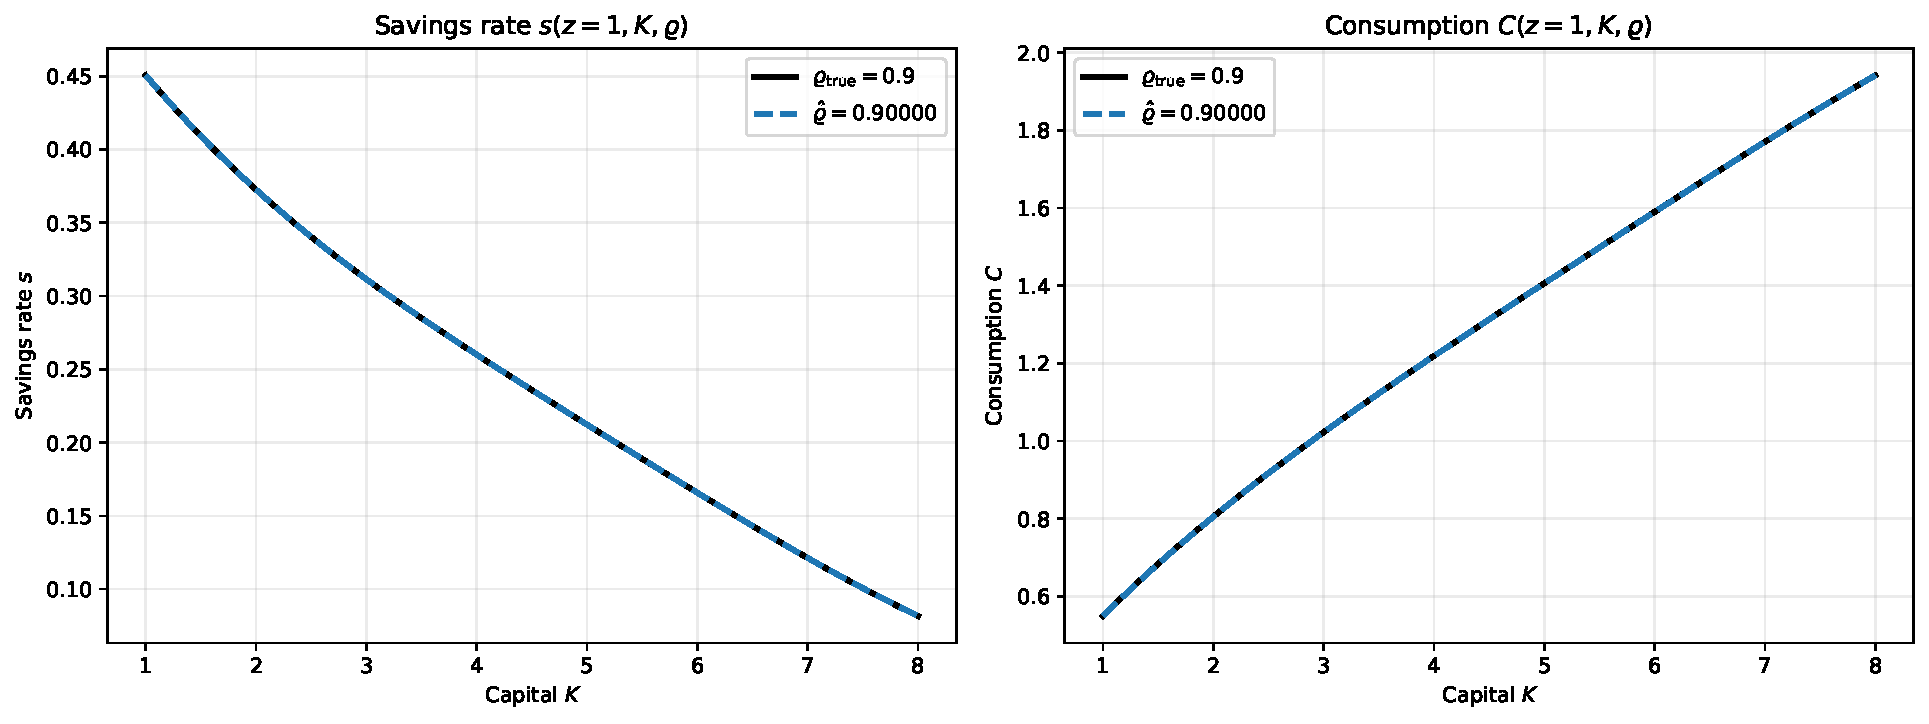
\includegraphics[width=0.85\textwidth]{rho_policy_comparison.pdf}
\end{center}
\vspace{-0.15cm}
\small
The estimated policy at $\hat\varrho$ overlaps the true policy at $\varrho_{\text{true}}=0.90$ to plotting accuracy. Single-parameter SMM with sharp identification recovers the truth accurately under CRN.
\end{frame}

% =====================================================================
% PART B: joint (beta, persistence) exercise
% =====================================================================
\begin{frame}{Bridge: From Just-Identified to Joint}
\small
The single-parameter exercise is the cleanest version of the SMM workflow. But two real lessons remain:
\begin{itemize}
\itemsep1pt
  \item How does the surrogate scale to \emph{multiple} parameters? Same idea: add them as pseudo-states.
  \item What does the SMM criterion look like when one parameter is \emphc{partially identified}?
\end{itemize}
\vspace{0.1cm}
Notebook \texttt{03b} re-trains the surrogate on the rectangle $\beta \in [0.92, 0.99] \times \varrho \in [0.50, 0.99]$ and estimates both jointly.

\vspace{0.2cm}
Two moment subsets:
\begin{itemize}
  \item \emphc{Just-identified} (2 moments): $\{$ mean savings, $\mathrm{Corr}(\Delta\log C)\}$.
  \item \emphc{Over-identified} (4 moments): adds $\mathrm{Std}(\Delta\log C)$ and $\mathrm{Corr}(\log Y)$.
\end{itemize}
\end{frame}

\begin{frame}{Joint Task: Estimate $(\beta, \varrho)$}
\begin{block}{Goal}
$\hat\theta = \argmin_{\theta = (\beta,\varrho)}\; [m(\theta) - \hat{m}^{\mathrm{data}}]^\top W\, [m(\theta) - \hat{m}^{\mathrm{data}}]$ \quad on $\beta\in[0.92,0.99] \times \varrho\in[0.50, 0.99]$.
\end{block}
\begin{enumerate}
  \itemsep1pt
  \item 4-input MLP $(z, K, \beta, \varrho) \to s$. Train once on the whole rectangle.
  \item Forge synthetic data at $(\beta_{\text{true}}, \varrho_{\text{true}}) = (0.96, 0.90)$.
  \item Compute the SMM criterion on a $25\times 25$ grid in $(\beta, \varrho)$ -- visualize both moment subsets.
  \item Refine with \texttt{scipy.optimize.minimize} (\texttt{L-BFGS-B}, which honours the box constraints natively, started from the grid argmin).
  \item Verify the solution is interior; report distance to truth on each axis.
\end{enumerate}
\end{frame}

% --- New frame: BoTorch UCB acquisition ---
\begin{frame}{BoTorch UCB Acquisition for Joint Estimation}
\textbf{Why active learning here.} On the 2D rectangle, most of the area sits far from the SMM minimiser -- pure exploration is wasteful. We want a design that hits both the basin of attraction \emphc{and} regions where the moment GP is uncertain.

\smallskip
\textbf{Acquisition function} (notebook 03b):
\[
a(\theta) \;=\; \bigl[\,0.25 + \widetilde{\mathrm{UCB}}_{g}(\theta)\,\bigr] \cdot \Bigl\|\boldsymbol\sigma_m(\theta) / \widehat{\mathrm{sd}}(m)\Bigr\|_2.
\]

{\scriptsize
\begin{itemize}\itemsep0pt
  \item $g(\theta) = -\log_{10}(Q(\theta) + \epsilon)$ is the negative log-criterion (a GP is fit to $g$); $\widetilde{\mathrm{UCB}}_g$ is BoTorch's standard $\mu_g + \kappa\sigma_g$ rescaled to $[0,1]$ over the grid.
  \item $\boldsymbol\sigma_m(\theta) \in \mathbb{R}^{n_m}$ stacks the moment-GP posterior std-deviations; $\widehat{\mathrm{sd}}(m)$ is the empirical std-deviation of each moment in the design (a unit-normaliser).
  \item $0.25$: a small floor on the exploit factor so candidates with low UCB on $g$ but high moment-GP uncertainty still enter the design.
\end{itemize}}

\smallskip
{\small\textbf{Roles.} First factor = \emph{exploit} (basin of small $Q$); second factor = \emph{explore} (where moment GPs are uncertain). Pure UCB on $g$ alone would over-collapse to the basin; pure moment-uncertainty would ignore the criterion shape.}

\medskip
{\scriptsize Built on BoTorch \texttt{SingleTaskGP} + \texttt{UpperConfidenceBound}; the multiplicative form is custom (not a stock BoTorch acquisition).}
\end{frame}

\begin{frame}{Expected Result: Surrogate Slices on $(\beta, \varrho)$}
\begin{center}
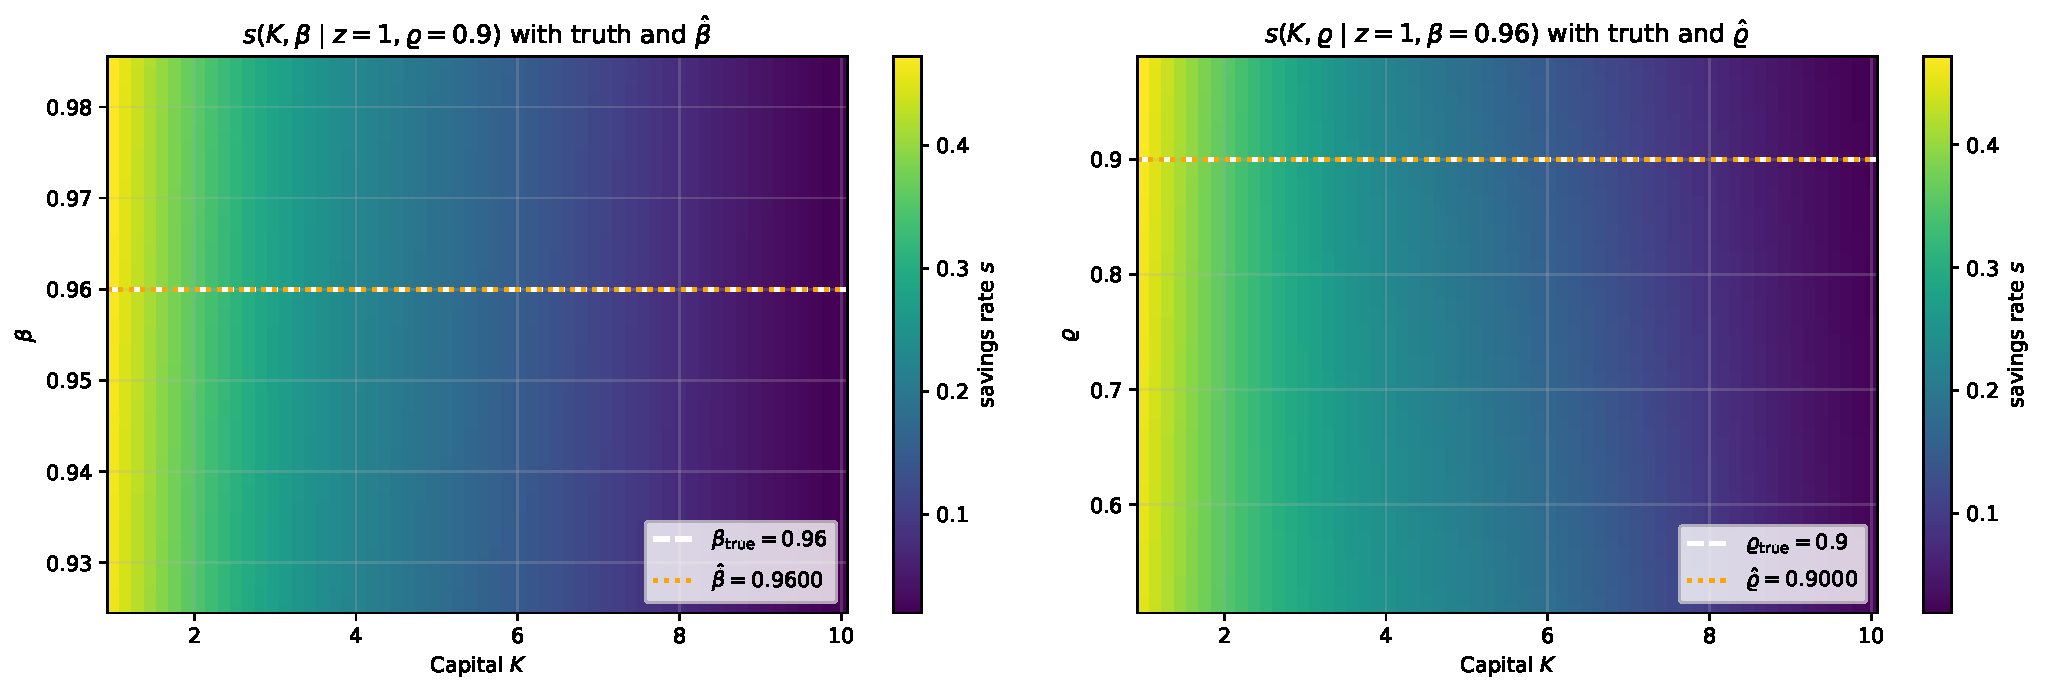
\includegraphics[width=0.95\textwidth]{joint_surrogate_with_estimates.pdf}
\end{center}
\vspace{-0.1cm}
\small
Two slices of the same 4-input network. White dashed = truth, orange dotted = over-identified estimate. The estimate sits strictly \emphc{inside} the rectangle on both axes simultaneously.
\end{frame}

\begin{frame}{Expected Result: 2D SMM Criterion}
\begin{center}

\includegraphics[width=0.95\textwidth]{joint_criterion_contour.pdf}
\end{center}
\vspace{-0.15cm}
\small
Left: the just-identified criterion shows a \emphc{ridge} along $\beta$ -- exactly the partial-identification problem that motivates calibrating $\beta$ in practice. Right: adding two persistence moments collapses the ridge to a localized minimum.
\end{frame}

% --- New frame: GP surrogate of the SMM criterion ---
\begin{frame}{GP Surrogate of the SMM Criterion}
\begin{center}
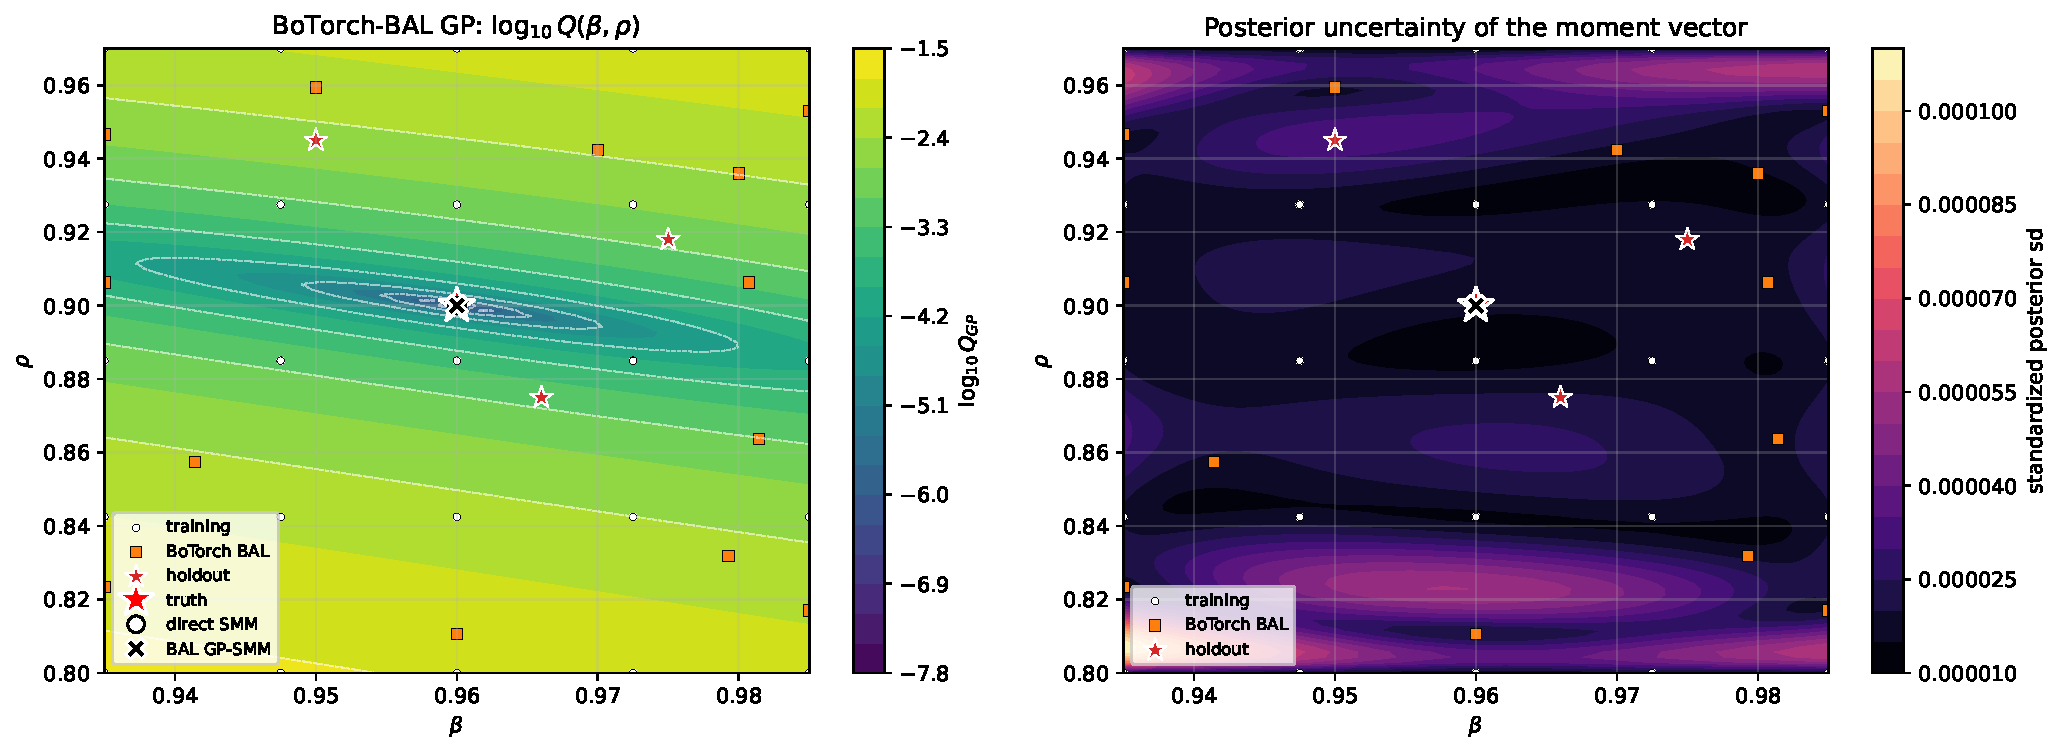
\includegraphics[width=0.72\textwidth]{fig/joint_gp_objective_surrogate.pdf}
\end{center}
\vspace{-0.15cm}
\scriptsize
\begin{itemize}\itemsep0pt
\item Left: GP posterior mean of $\log_{10} Q(\beta,\varrho)$; right: standardized moment uncertainty.
\item White dots = training design; orange squares = active additions; red stars = holdouts/truth.
\item White circle = direct SMM; black cross = GP-SMM. Later objective calls need only one GP posterior evaluation.
\end{itemize}
\end{frame}

\begin{frame}{Expected Result: Estimates on Top of Criterion}
\begin{center}
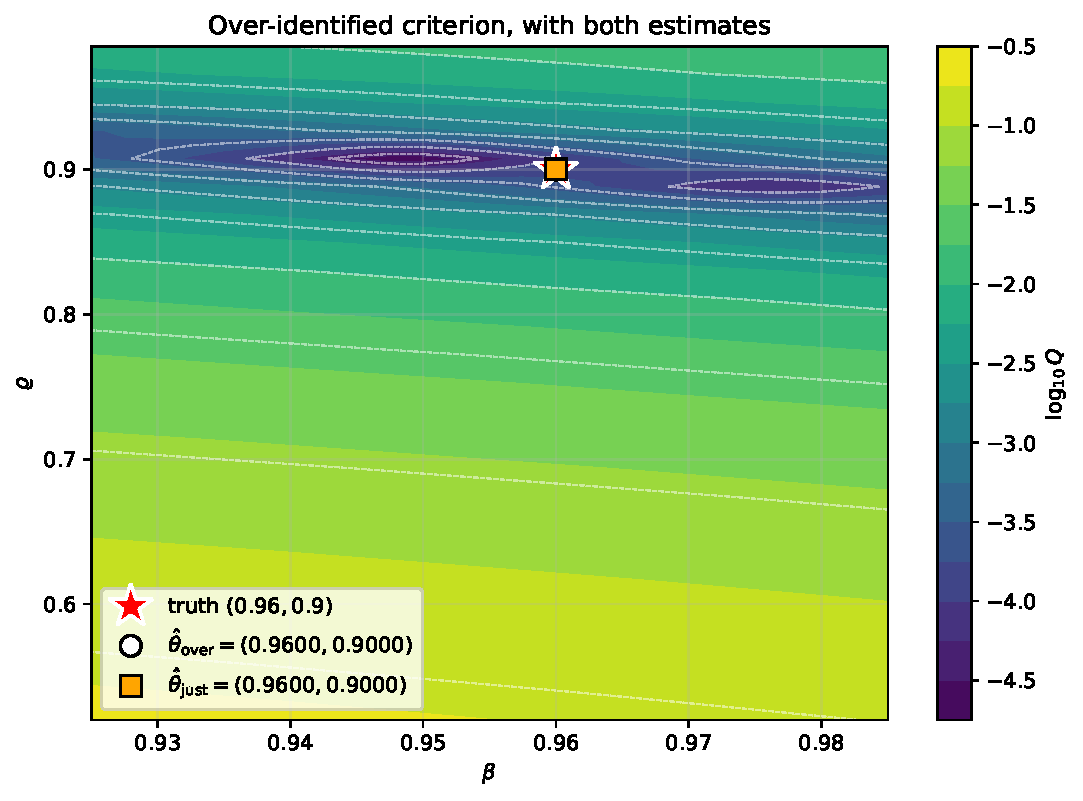
\includegraphics[width=0.55\textwidth]{joint_estimates_overlay.pdf}
\end{center}
\vspace{-0.2cm}
\scriptsize
In this synthetic CRN run, both estimators recover $(\beta,\varrho)$ close to the truth. The takeaway is the criterion's \emph{shape}: the just-identified ridge would translate into wide confidence bands on $\beta$ in real-data applications, while the over-identified criterion has localized curvature on both axes.
\end{frame}

\begin{frame}{Joint Policy Match}
\begin{center}
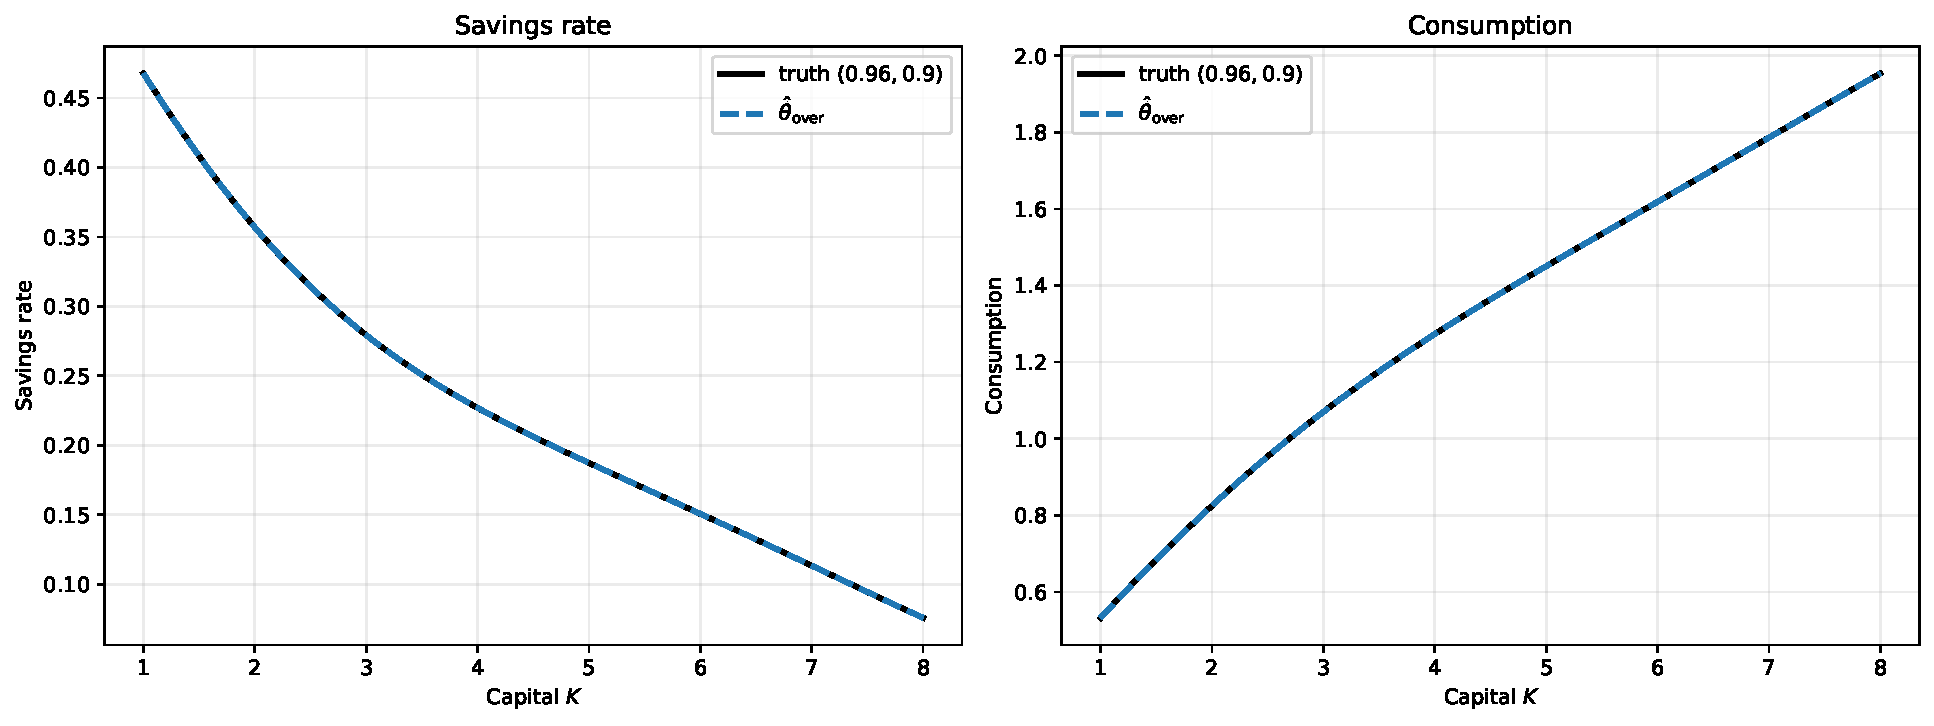
\includegraphics[width=0.85\textwidth]{joint_policy_comparison.pdf}
\end{center}
\vspace{-0.1cm}
\small
Savings rate and consumption at the over-identified estimate overlay the truth almost exactly. The 4-input surrogate, trained \emph{once}, supports millions of cheap moment evaluations during the optimizer's line-search.
\end{frame}

\begin{frame}{Wrap-Up}
\small
What the two notebooks teach together:
\begin{itemize}
\itemsep1pt
  \item A neural surrogate with parameters as pseudo-states \emphc{decouples} the cost of solving the structural model from the cost of moment-matching. Train once, use it inside any optimizer.
  \item For a well-identified parameter ($\varrho$), SMM under CRN gives a sharp 1D identification picture.
  \item For \emphc{joint} estimation, the contour plot makes the partial-identification ridge visible. Adding moments collapses it.
  \item The \emphc{interior-solution} check is part of the standard pipeline, needed for the asymptotic distribution theory of the SMM estimator.
\end{itemize}
\vspace{0.10cm}
{\footnotesize \textbf{Formal identification machinery} (moment Jacobian $M = \partial m/\partial\theta$, rank condition, $J$-statistic, weak-identification diagnostics): see lecture script Sec. 10.4 (Practical Considerations).}
\vspace{0.10cm}\\
\textbf{Production pipeline:} Chen, Didisheim \& Scheidegger (2026, \emph{J.\ Financial Economics}), exactly this surrogate-and-SMM logic at scale, applied to finance.
\end{frame}

\end{document}
